\documentclass{article}
\usepackage[utf8]{inputenc}
\usepackage[spanish]{babel}
\usepackage[]{amsthm}
\usepackage{amsmath}
\usepackage[]{amssymb}
\usepackage{graphicx}
\usepackage{wrapfig}
\usepackage[letterpaper, margin=1.5in]{geometry}
\usepackage[hidelinks]{hyperref}
\decimalpoint

\begin{document}
    \begin{titlepage}
        \begin{center}
            \begin{figure}
                \centering
                \includegraphics[scale=0.13]{img/logo_itesm.png}\\ % Logo de la institución
            \end{figure}
        \vspace{5cm}
        \LARGE{Instituto Tecnológico y de Estudios Superiores de Monterrey}\\
        \fontsize{12}{14}\selectfont
        \vspace{1cm}
        \textbf{Actividad 3.2.2.1 Creación del laboratorio de pruebas}\\ % Nombre de la tarea
        \vspace{0.7cm}
        \begin{table}[h!]
            \centering
            \begin{tabular}{ ||c|c|| }
                \hline
                Nombre & Matrícula \\
                \hline
                Juan Pablo Echeagaray González & A00830646 \\
                \hline
                Verónica Victoria García De la Fuente & A00830383 \\
                \hline
                Emmanuel Isaí Godínez Flores & A01612966 \\
                \hline
                Carlos David Lozano Sanguino & A01275316 \\
                \hline
                Emily Rebeca Méndez Cruz & A00830768 \\
                \hline
                Eugenio Santisteban Zolezzi & A01720932 \\
                \hline
            \end{tabular}
        \end{table}
        \vspace{0.7cm}
        Aplicación de criptografía y seguridad\\ % Materia
        \vspace{0.2cm}
        MA2005B.201\\ % Clave de la materia
        \vspace{0.2cm}
        Dr. Alberto Francisco Martínez Herrera\\ % Nombre del profesor
        \vspace{0.2cm}
        Dr. Oscar Eduardo Labrado Gómez \\
        \vspace{0.7cm}
        28 de septiembre del 20222\\ % Fecha de entrega
        \end{center}
    \end{titlepage}

    \tableofcontents
    \clearpage

    \section{Introducción}
        
        Para fines de la elaboración del reto de la materia \emph{Aplicación de criptografía y seguridad} se ha creado un entorno virtual en la computadora de cada uno de los miembros de este equipo. Se ha seguido una guía provista por los profesores responsables de la materia; dicha guía presenta instrucciones detalladas para la instalación de software de virtualización que simulará una red local compuesta de una máquina que fungirá como un servidor que brinda conexión a varias computadoras cliente locales.

    \section{Metodología}

        \subsection{Instalación de herramienta de virtualización}

            El equipo ha decidido usar en conjunto el software \emph{VirtualBox} de la empresa \emph{Oracle} \cite{vbox-doc}. La aplicación puede ser descargada del sitio oficial \href{https://www.virtualbox.org/wiki/Downloads}{aquí}.

            La versión usada para este entregable es \texttt{6.1.38}, se han utilizado sus versiones para los sistemas operativos \emph{Windows-OS} y \emph{Linux}.

            Una vez instalada la aplicación, el usuario verá una ventana similar a la presentada en la figura \ref{fig:fresh-vbox}.

        \subsection{Instalación de Kali-Linux} \label{sec:kali-install}

            Una vez descargado \emph{VirtualBox} se procede a descargar la máquina virtual de \emph{Kali-Linux} de \href{https://www.kali.org/get-kali/#kali-virtual-machines}{este} sitio. El equipo ha descargado la versión de 64-bits apropiada para \emph{VirtualBox}. Una vez que se haya completado la descarga, se descomprime el archivo para añadirlo a la interfaz de la aplicación.

            Para agregar la máquina virtual se va a \texttt{File > Import Appliance} y se selecciona el archivo \texttt{.vbox} que se encuentra en la carpeta que acabamos de descomprimir. En esta etapa no se modificarán ninguno de los valores predeterminados. Para comenzar a usar la máquina podemos simplemente hacer doble-click en el nuevo ícono que tendremos en el menú, las credenciales de este equipo son:
            \begin{itemize}
                \item Username: \texttt{kali}
                \item Password: \texttt{kali}
            \end{itemize}

            Al realizar estos pasos con éxito se verá una máquina como la de la figura \ref{fig:kali-init}.

        \subsection{Instalación de Windows}

            El siguiente paso en esta guía es la instalación de una máquina virtual con sistema operativo \emph{Windows 10}, dicha máquina puede ser descargada del siguiente \href{https://developer.microsoft.com/en-us/microsoft-edge/tools/vms/}{enlace}. Para nuestro caso descargaremos la máquina virtual \texttt{MSEdge on Win10 (x64) Stable 1809} para la plataforma \emph{VirtualBox} como se ve en la figura \ref{fig:windows-download}.

            Ya que se descomprima el archivo \texttt{.zip} descargado se seguirá el mismo procedimiento que el descrito en la sección \ref{sec:kali-install}, yendo a la ruta \texttt{File > Import Appliance} y seleccionando el archivo \texttt{.ova} generado en la carpeta descomprimida; una vez más no se recomienda modificar los valores por defecto. De realizar estos pasos con éxito, el usuario podrá iniciar sesión con las siguientes credenciales:
            \begin{itemize}
                \item Username: \texttt{IEUser}
                \item Password: \texttt{Passw0rd!}
            \end{itemize}

            Al iniciar sesión el usuario verá una pantalla como la de la figura \ref{fig:windows-init}.

        \subsection{Instalación de Metasploitable}

            Ahora se procede a descargar una máquina virtual de \emph{Metasploitable} del siguiente \href{https://sourceforge.net/projects/metasploitable/}{enlace}. Al descomprimir el archivo \texttt{.zip} se encontrará un directorio con los contenidos presentes en la figura \ref{fig:meta-download}.

            Se añade ahora una nueva máquina virtual por la ruta \texttt{Machine > New}, el tipo de máquina es \texttt{Linux} y la versión es \texttt{Ubuntu 64bits} como se ve en la figura \ref{fig:meta-create}.

            En la sección de disco duro hay que escoger la opción de utilizar un disco duro virtual existente. Aquí cargaremos el archivo \texttt{.vmdk} que se encuentra en la carpeta que descomprimimos al comienzo de este paso. Al cargar ese archivo y continuar con los valores por defecto de instalación podremos instalar la máquina. Iniciaremos sesión en ella con las credenciales:
            \begin{itemize}
                \item Username: \texttt{msfadmin}
                \item Password: \texttt{msfadmin}
            \end{itemize}

            Al iniciar sesión con éxito veremos una pantalla de consola como la de la figura \ref{fig:meta-init}.

        \subsection{Instalación de Ubuntu}

            Se procederá a descargar el archivo \texttt{.iso} del siguiente \href{https://releases.ubuntu.com/focal/}{enlace}, en particular es el que se presenta bajo el hipervínculo con el texto \texttt{64-bit PC (AMD64) desktop image}. Con este archivo ahora podemos instalar la máquina virtual.

            Crearemos una máquina nueva por la ruta \texttt{Machine > New}, el tipo de la máquina será \texttt{Linux} y la versión \texttt{Ubuntu 64 bits}. Se debe de proceder con la instalación con los valores por defecto, pero darle un tamaño de 30 GB.

            Después se enciende la máquina virtual, recibiremos una ventana como la de la figura \ref{fig:ubuntu-iso-load}, seleccionar aquí el archivo \texttt{.iso} que descargamos con anterioridad. Se continuará con el proceso de instalación, escogiendo la opción de \texttt{Install Ubuntu}, los valores por defecto no serán modificados y se seleccionará la opción de borrado del disco duro.

            Las credenciales de acceso así como el nombre de la máquina virtual quedan a libre elección del usuario, se recomienda que la zona horaria seleccionada sea la del usuario, permitirá darle una interpretación más sencilla a las actividades venideras.

            Cuando termine el proceso de instalación puede apagarse la máquina, para después seleccionarla en la ventana inicial de \emph{VirtualBox}, seguir la ruta \texttt{Settings > Storage > Controller: IDE}, seleccionar el disco que viene cargado con click-derecho y remover. Se tiene que dar \texttt{ok} en esa pantalla para que los cambios tengan efecto. Al realizar este paso para después arrancar la máquina e iniciar sesión con las credenciales configuradas, el usuario podrá ver una ventana como la de la figura \ref{fig:ubuntu-init}.

        \subsection{Instalación de pfSense}
            
            Se descarga ahora una máquina virtual desde la plataforma \texttt{pfSense} \href{https://www.pfsense.org/download/#}{aquí}. La configuración de la descarga será de arquitectura \texttt{AMD64}, el instalador es el de la versión \texttt{DVD Image}, el espejo es libre, aunque se recomienda escoger uno lo más cercano posible a la locación física del usuario.

            Cuando la descarga se complete, se descomprimirá el archivo para obtener uno con terminación \texttt{.iso}. Se añadirá una máquina nueva mediante la ruta \texttt{Machine > New}, el tipo de máquina es \texttt{BSD}, y la versión \texttt{FreeBSD (64-bit)}. Pueden no modificarse los valores por defecto, pero aquí se puede reducir el espacio máximo que necesite la VM, nosotros hemos optado por valores en el rango de 3 a 7 GB.

            Antes de seguir con los siguientes paso modificaremos la conexión que tendrá esta computadora al acceder por la ruta \texttt{Settings > Network > Adapter 1}. Lo modificaremos de NAT a \texttt{Bridged Adapter} como se ve en la figura \ref{fig:pfsense-bridged-adapter}.

            Se cargará ahora el archivo \texttt{.iso} descargado mediante la ruta \texttt{Settings > Storage > Controller: IDE > Empty}, en el ícono de disco azul que aparece en la figura \ref{fig:pfsense-iso-load} se podrá cargar dicho archivo \texttt{.iso}.

            Se arrancará la VM para iniciar el proceso de instalación. Comenzamos por dar \texttt{Accept} a la pantalla de inicio, después se dará \texttt{OK} para proceder con la instalación, recalcamos que debe de estar seleccionada la opción \texttt{Install}. Los valores por defecto no serán modificados, pero se recomienda después escoger la opción \texttt{Auto (UFS) BIOS option}, cuando termine el proceso de instalación se seleccionará la opción \texttt{NO} para seleccionar después \texttt{Reboot}, en cuando reinicie el sistema, presionar la tecla \texttt{ESC} y apagar la máquina virtual.

            Ahora se expulsará el archivo \texttt{.iso} que se cargó con anterioridad en la ruta \texttt{Settings > Storage > Controller: IDE}, seleccionar el archivo que ahora se verá en esa pantalla, y hacer click en \texttt{Remove attachment}. Hecho esto, se irá a la sección \texttt{Network}, para crear una red interna que compartirán las demás máquinas virtuales, se seleccionará y habilitará el adaptador 2 en modo de conexión interna, el nombre de la red queda a criterio del usuario. Se debe de tener una configuración como la de la figura \ref{fig:pfsense-internal}.

            Iniciar ahora la máquina virtual, este proceso tomará algo de tiempo, pero se debe de llegar a una ventana como la de la figura \ref{fig:pfsense-init}. \textbf{No apagar la máquina virtual ahora}.
        
        \subsection{Configuración de redes}

            Para cada una de las máquinas virtuales previamente instaladas, a excepción del router, acceder a la configuración de la red por la ruta \texttt{Settings > Network > Adapter 1}, modificar sus valores para que la red a utilizar sea la red interna previamente creada, debe de quedar un resultado como el de la figura \ref{fig:all-internal}.

        \subsection{Configuración del router} \label{sec:router-config}

            Encender la máquina virtual de su elección para configurar el router previamente creado, recomendamos que sea una que posea una interfaz gráfica. Acceder al navegador que tenga a su disposición, y escribir en la barra de búsqueda el IP asignado al router, este puede obtenerse al usar el comando \texttt{ipconfig} en la máquina \texttt{pfsense}, si se siguieron los pasos aquí descritos, la IP asignada será \texttt{192.168.1.1}.

            Iniciar sesión con las credenciales:
            \begin{itemize}
                \item Username: admin
                \item Password: pfsense
            \end{itemize}

            Se verá ahora una ventana como la de la figura \ref{fig:pfsense-config-init}. Proceda con el proceso de instalación sin modificar los valores por defecto. Al terminar seleccione el botón de aplicar cambios.

            Cuando se termine este proceso, el router habrá sido configurado, puede comprobar en cada una de las máquinas que exista una conexión a internet; un ejemplo de este resultado puede observarse en la figura \ref{fig:all-internet}.

    \section{Notas}

        Como equipo hemos encontrado algunas posibles razones por las que los pasos anteriores no podrían ser exitosos, para cada uno de ellos proveemos algunos posibles arreglos que nos han funcionado durante la realización de esta tarea:
        \begin{itemize}
            \item Fallo en asignación de IP a red WAN en pfSense: Un posible origen de esta problemática es la configuración del router al que se conecta nuestra computadora principal (la que corre VirtualBox), sugerimos seguir esta metodología con una conexión diferente.
            \item Fallo en resolución de nombres al usar comando ping: Al seguir con los valores por defecto de la configuración de \texttt{pfSense} podría presentarse el caso de que el \texttt{DNS Resolver} de fábrica no logre brindar una conexión de internet a las máquinas virtuales, para resolver este problema será necesario hacer un \texttt{reset} del router para configurar un \texttt{DNS Resolver} funcional, la guía descrita en el siguiente \href{https://coygeek.com/docs/pfsense-virtualbox/}{link} provee pasos detallados sobre las modificaciones que deben hacerse en la configuración del router que describimos en la sección \ref{sec:router-config}
        \end{itemize}
    
    \section{Imágenes}

        \begin{figure}[!htbp]
            \centering
            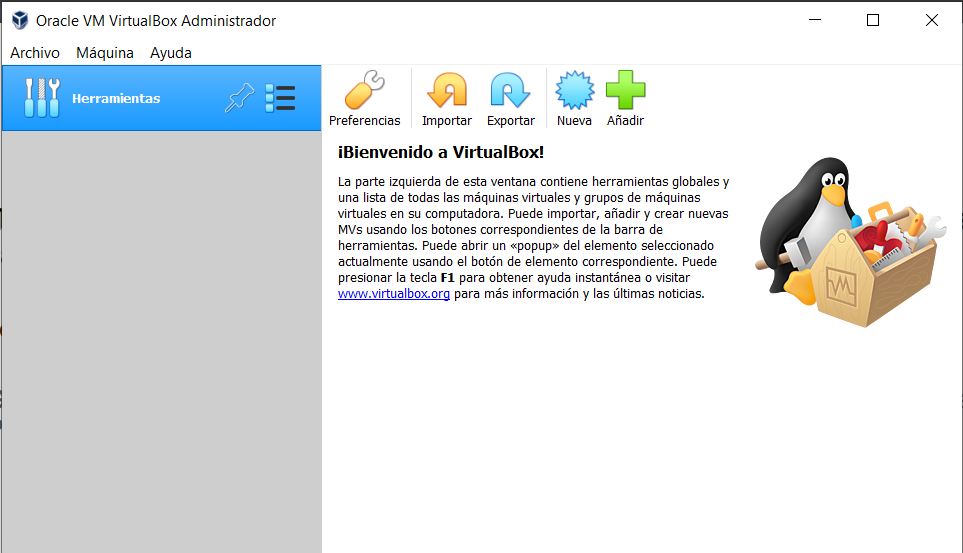
\includegraphics[scale=0.25]{img/virtual-box.png}
            \caption{Ventana de bienvenida de VirtualBox}
            \label{fig:fresh-vbox}
        \end{figure}

        \begin{figure}[!htbp]
            \centering
            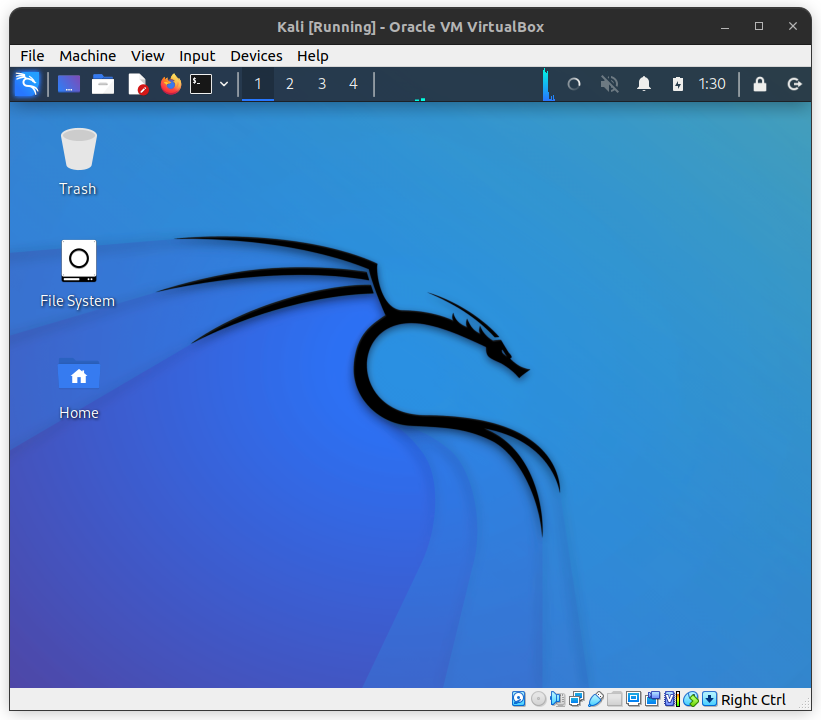
\includegraphics[scale=0.25]{img/kali-screen.png}
            \caption{Ventana de inicio de Kali}
            \label{fig:kali-init}
        \end{figure}

        \begin{figure}[!htbp]
            \centering
            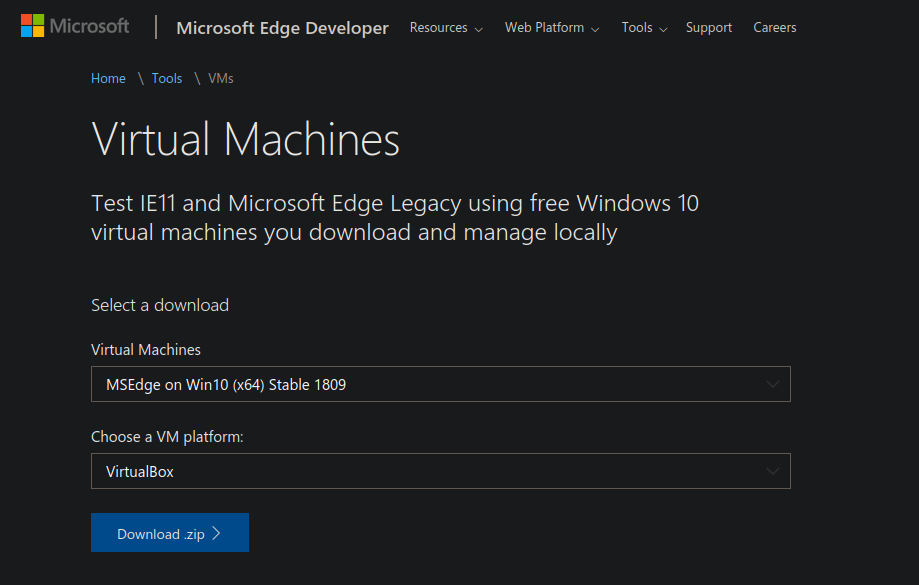
\includegraphics[scale=0.3]{img/win-download.png}
            \caption{Descarga de máquina virtual con Windows 10}
            \label{fig:windows-download}
        \end{figure}

        \begin{figure}[!htbp]
            \centering
            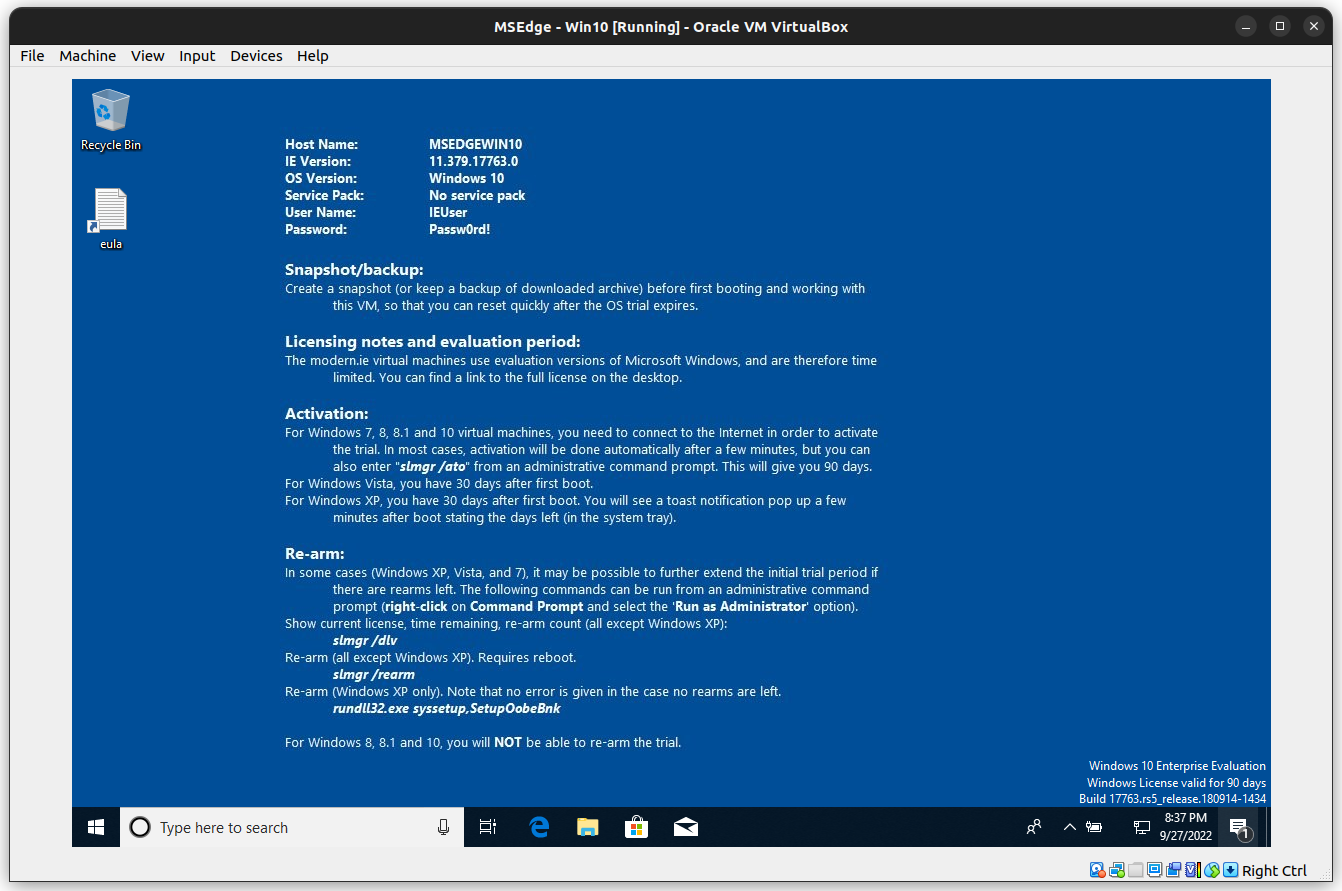
\includegraphics[scale=0.2]{img/windows-init.png}
            \caption{Pantalla de inicio de Windows}
            \label{fig:windows-init}
        \end{figure}

        \begin{figure}[!htbp]
            \centering
            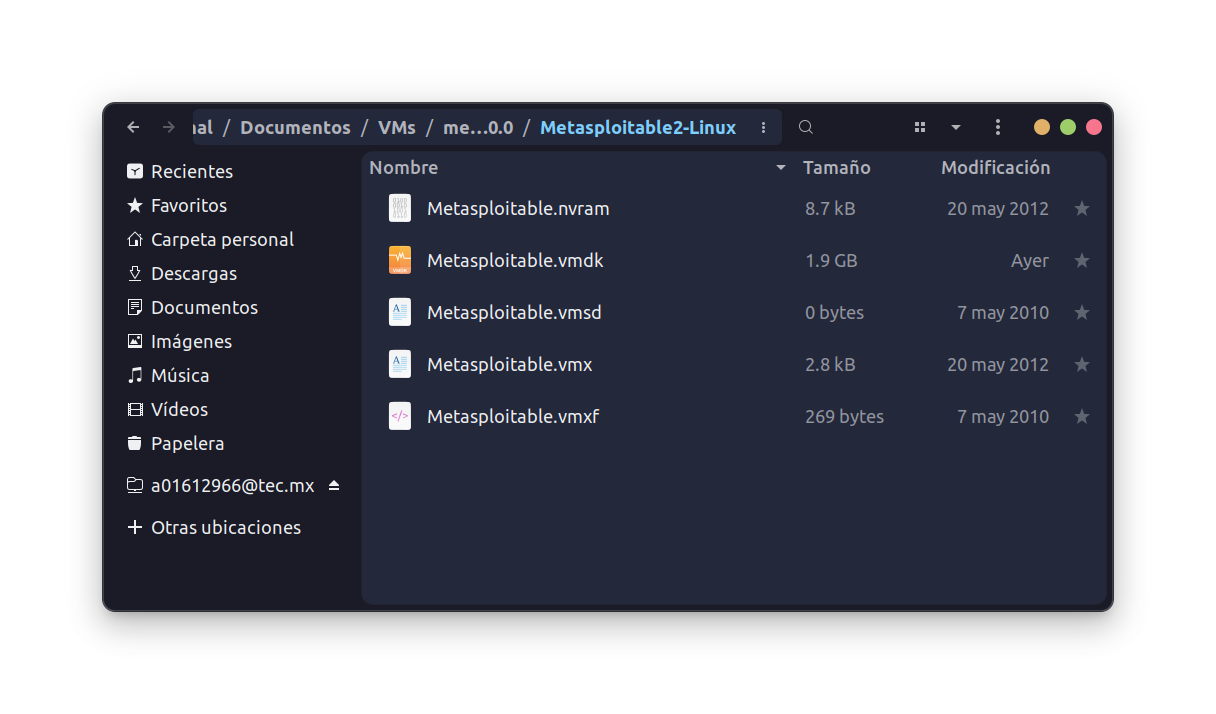
\includegraphics[scale=0.2]{img/meta-download.png}
            \caption{Archivos descargados de Metasploitable}
            \label{fig:meta-download}
        \end{figure}

        \begin{figure}[!htbp]
            \centering
            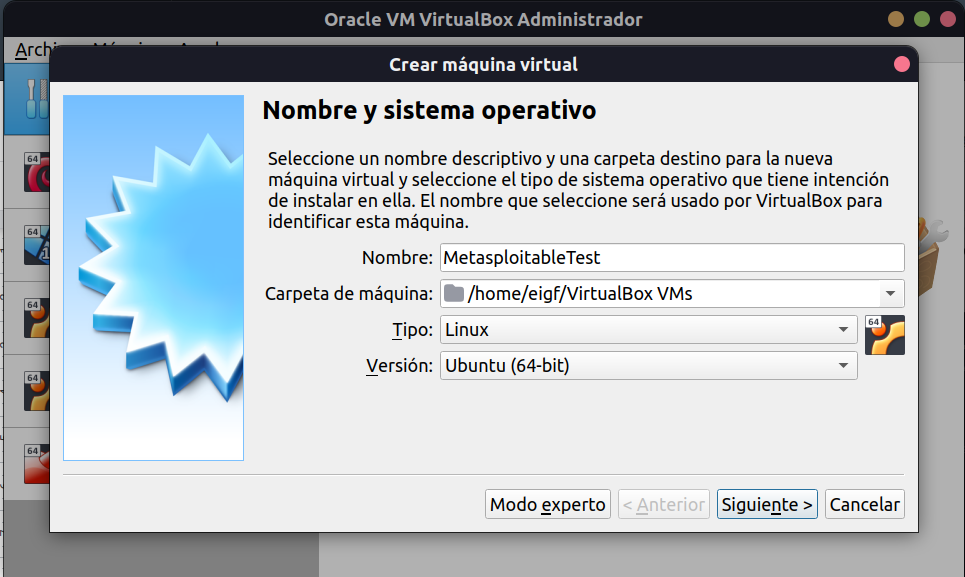
\includegraphics[scale=0.25]{img/meta-create.png}
            \caption{Creación de máquina virtual Metasploitable}
            \label{fig:meta-create}
        \end{figure}

        \begin{figure}[!htbp]
            \centering
            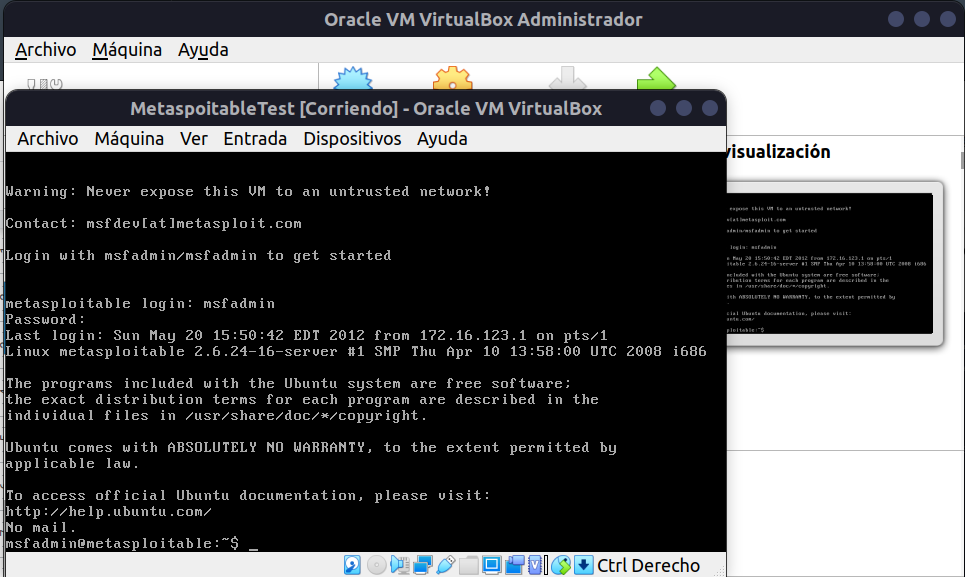
\includegraphics[scale=0.3]{img/meta-init.png}
            \caption{Ventana de inicio de Metasploitable}
            \label{fig:meta-init}
        \end{figure}

        \begin{figure}[!htbp]
            \centering
            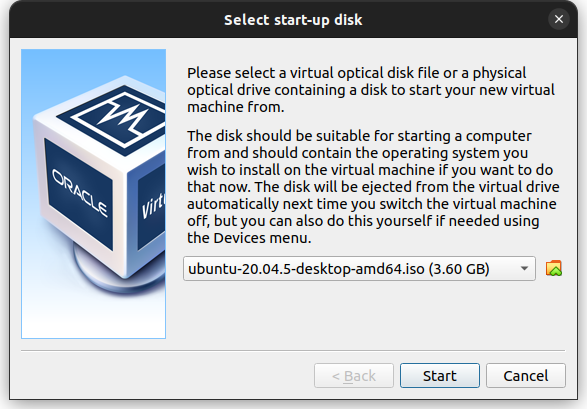
\includegraphics[scale=0.4]{img/ubuntu-install.png}
            \caption{Carga de archivo de instalación .iso de Ubuntu}
            \label{fig:ubuntu-iso-load}
        \end{figure}

        \begin{figure}[!htbp]
            \centering
            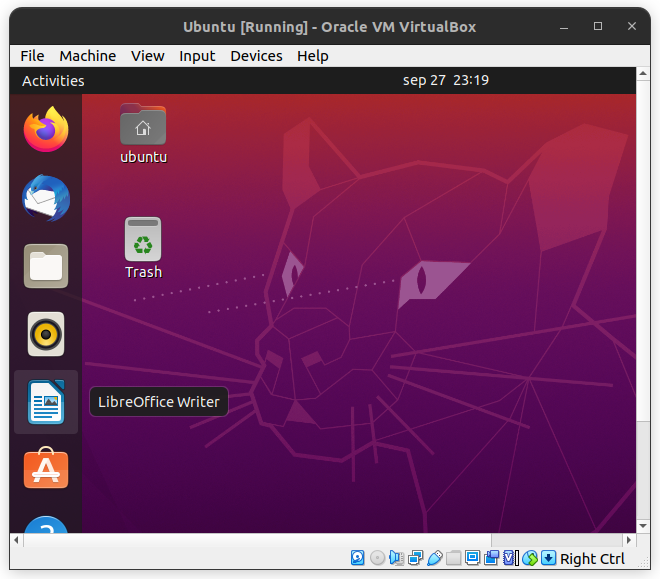
\includegraphics[scale=0.4]{img/ubuntu-init.png}
            \caption{Ventana de inicio de Ubuntu}
            \label{fig:ubuntu-init}
        \end{figure}

        \begin{figure}[!htbp]
            \centering
            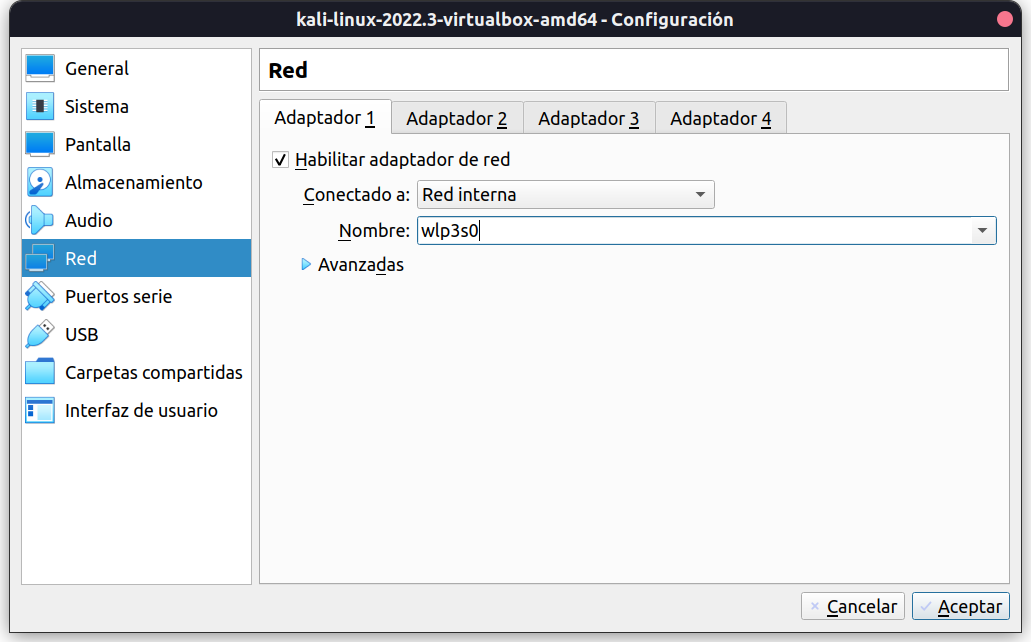
\includegraphics[scale=0.3]{img/pfsense-bridged-adapter.png}
            \caption{Modificación a red Bridged en Router}
            \label{fig:pfsense-bridged-adapter}
        \end{figure}

        \begin{figure}[!htbp]
            \centering
            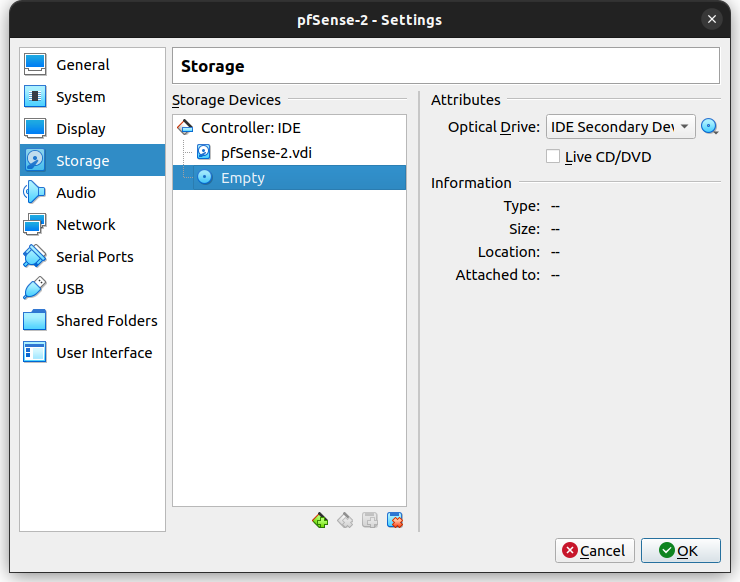
\includegraphics[scale=0.3]{img/pfsense-iso-load.png}
            \caption{Carga de archivo .iso}
            \label{fig:pfsense-iso-load}
        \end{figure}

        \begin{figure}[!htbp]
            \centering
            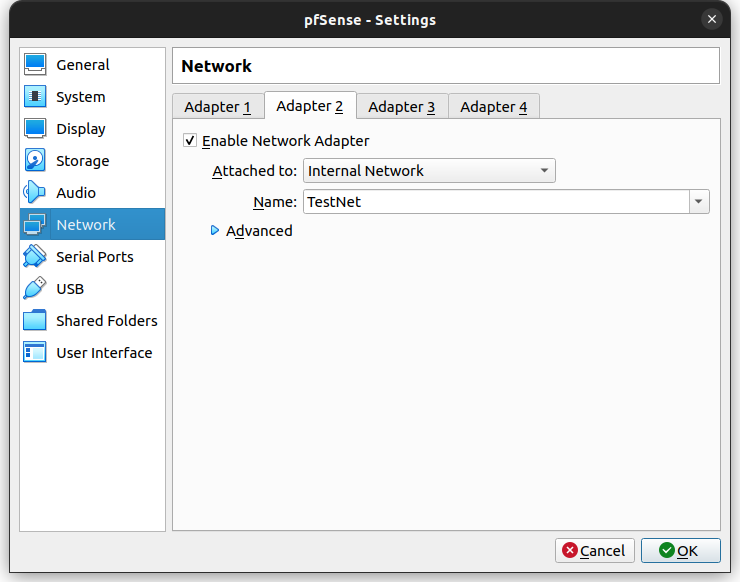
\includegraphics[scale=0.3]{img/pfsense-internal.png}
            \caption{Creación de red interna}
            \label{fig:pfsense-internal}
        \end{figure}

        \begin{figure}[!htbp]
            \centering
            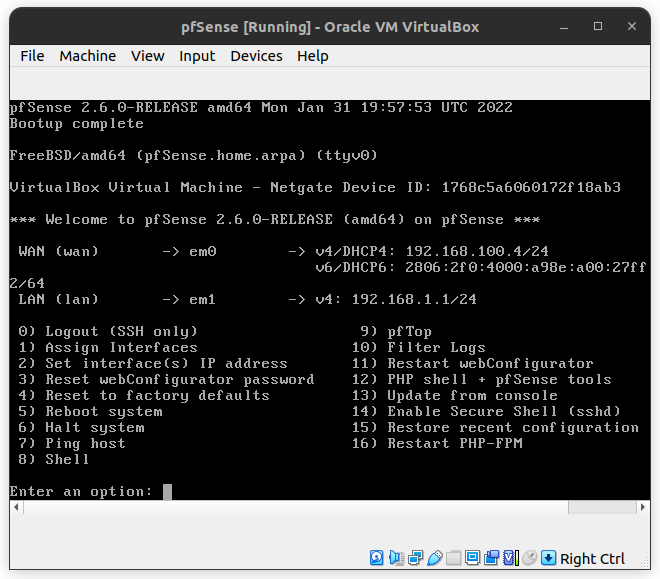
\includegraphics[scale=0.3]{img/pfsense-init.png}
            \caption{Ventana de inicio de pfSense}
            \label{fig:pfsense-init}
        \end{figure}

        \begin{figure}[!htbp]
            \centering
            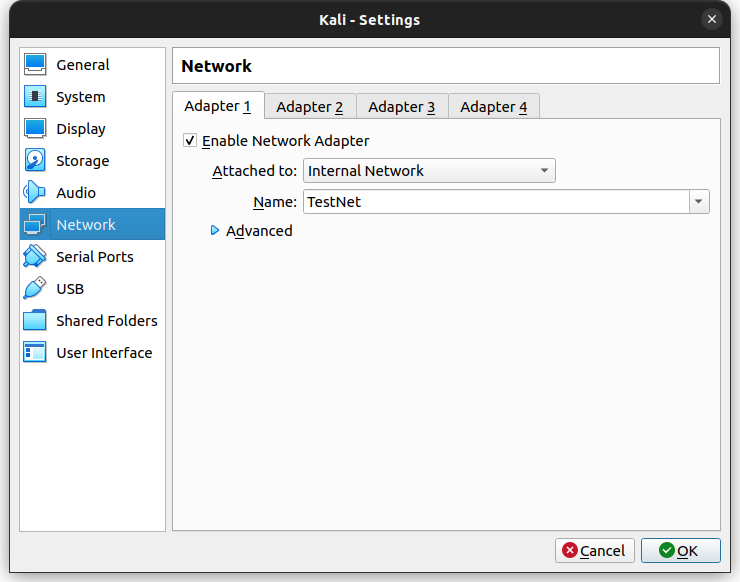
\includegraphics[scale=0.25]{img/all-internal.png}
            \caption{Configuración de red interna}
            \label{fig:all-internal}
        \end{figure}

        \begin{figure}[!htbp]
            \centering
            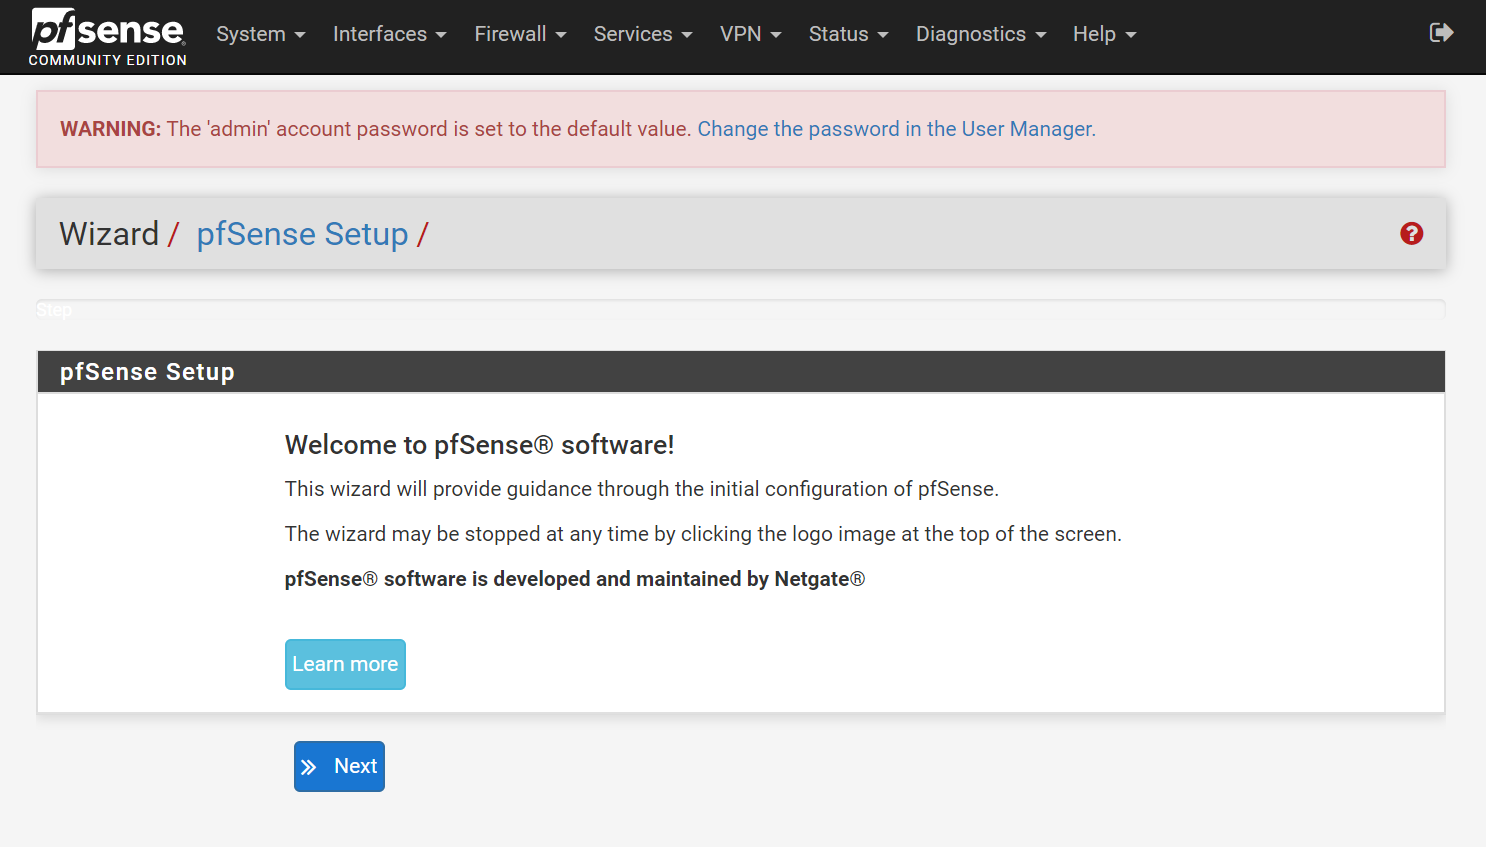
\includegraphics[scale=0.3]{img/pfsense-config-init.png}
            \caption{Ventana inicial de configuración del router}
            \label{fig:pfsense-config-init}
        \end{figure}

        \begin{figure}[!htbp]
            \centering
            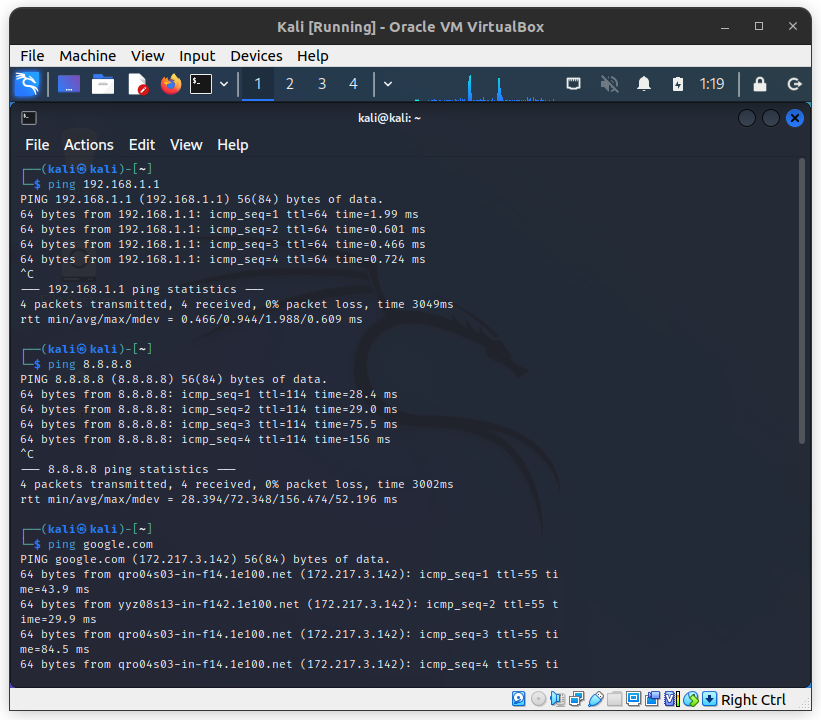
\includegraphics[scale=0.3]{img/all-internet.png}
            \caption{Conexión a internet exitosa}
            \label{fig:all-internet}
        \end{figure}
        
    \clearpage
    \bibliographystyle{IEEEtran}
    \bibliography{references.bib}

\end{document}